\documentclass[12pt]{article}

% for footnotes
\makeatletter
\newcommand\footnoteref[1]{\protected@xdef\@thefnmark{\ref{#1}}\@footnotemark}
\makeatother

\usepackage{common}
\usepackage{macros}
\usepackage{nameref}
\usepackage{pdflscape}

\title{HW1: Classification}
\author{Jiafeng Chen \and
Francisco Rivera}
\begin{document}

\maketitle{}
\section{Introduction}
In this write-up, our main focus is language modeling. That is, given words in a
sentence, can we predict the word that follows? We implemented a
\nameref{subsec:trigram}, a embedding neural network model, an
\nameref{subsec:lstm}, and a few extensions---including pre-trained embeddings,
ensemble models, and multi-head attention decoders.

\section{Problem Description}


To tackle language modeling, we start with sequences of words $w \in \mcV$ in
some vocabulary $\mcV$ and aim to predict the last word in the sequence which we
cannot observe. We can do this probabilistically by attempting to estimate,
\begin{equation}
p(w_t \mid w_1, \ldots, w_{t-1})
\label{eq:probabilistic}
\end{equation}
that is, the conditional distribution over the last word conditional on the
words leading up to it.

In particular, there will be a special word, $w_\text{unk} \in \mcV$ which
represent an unknown word; we use this whenever we encounter a token we have not
previously seen.

In some models, we represent words with dense embeddings. That is, each word
gets assigned a vector $\boldv \in \mathbb{R}^d$ where $d$ is the embedding
dimension. These embeddings are trained as part of the model, but can also be
initialized to pre-trained values.

\section{Model and Algorithms}


\subsection{Trigram model}
\label{subsec:trigram}

In our trigram model, we aim to estimate the probability written in Equation
\ref{eq:probabilistic}. This conditional probability is intractable itself
because it's likely that we've never seen the exact sequence of words $w_1,
\ldots, w_{t-1}$. However, we can gain tractability by dropping words toward the
beginning of the sequence, hoping that they don't affect the probability too
much. That is, we hope that,
\[ p(w_t \mid w_1, \ldots, w_{t-1}) \stackrel{?}{\approx} p(w_t \mid w_{t-2},
w_{t-1}).\]
Having replaced our first probability with a simpler one which conditions on
less information, we can estimate the latter by its empirical sample estimator.
In other words, we can take all the times in our training set when we've seen
words $w_{t-2}, w_{t-1}$ adjacent to each other, and consider the empirical
distribution of the word that follows them. We represent this sample
approximation as $\hat{p}$ and write,
\[ p (w_t \mid w_{t-2}, w_{t-1}) \approx \hat{p} (w_t \mid w_{t-2}, w_{t-1}).\]
By doing this, we've solved most of the intractability of conditioning on the
entire sentence $w_1, \ldots, w_{t-1}$, but we still have some of the same
problems. Namely, it's possible that in our training set, we either haven't seen
words $w_{t-2}$ and $w_{t-1}$ together before, or we've seen them only a very
small number of times such that the empirical probability distribution becomes a
poor approximation. (To avoid division by zero errors, we adopt the convention
that empirical probabilities are all 0 if we haven't seen the words being
conditioned on before.) We can fix this by also considering the probabilities,
\[ p(w_t) \text{ and } p(w_t \mid w_{t-1})\]
which give us the unconditional probability of a word and the probability
conditional on only the previous word. These have the benefit of being more
tractable to estimate and the drawback of losing information. In the end, we
calculate a blend of these three approximations:
\[ \alpha_1 \hat{p}(w_t \mid w_{t-2}, w_{t-1}) + \alpha_2
\hat{p}(w_t \mid w_{t-1}) + (1-\alpha_1-\alpha_2)\hat{p}(w_t).\]
Training the weights $(\alpha_1, \alpha_2)$ loads up most of our weight on
$\alpha_1$ which suggests the latter two probabilities are better used as
``tie-breakers'' when conditioning on the previous bi-gram yields a small number
of possibilities. In our final model, we use $(\alpha_1, \alpha_2) = (0.9,
0.05)$.

\subsection{Neural Network Language Model}
\label{sub:nnlm}
Following \cite{bengio2003neural}, we implement a neural network language model
(NNLM). We model \eqref{eq:probabilistic} by first assuming limited dependence: \[
p(w_i \mid w_1,\ldots,w_{i-1}) = p(w_i \mid w_{i-1}, \ldots, w_{i-k}),
\]
i.e., the current word only depends on the past $k$ words, a useful restriction
motivated by n-gram models. Next, we convert input tokens $w_{i-1},\ldots,w_
{i-k}$ into embedding vectors $\br{\boldv_{i-t}}_{t=1}^k$ and concatenate them
into a $dk$ vector $\bm v_{i-k:i-1}$. We then pass this vector into a
multilayer perceptron network with a softmax output into $|\mathcal V|$ classes.
We implement this efficiently across a batch by using a convolution operation,
since convolution acts like a moving window of size $k$. This way we can
generate $T - k + 1$ predictions for a sentence of length $T$. We depict the
convolution trick in \Cref{fig:nnlm}. 

\begin{figure}[tb]
    \centering
    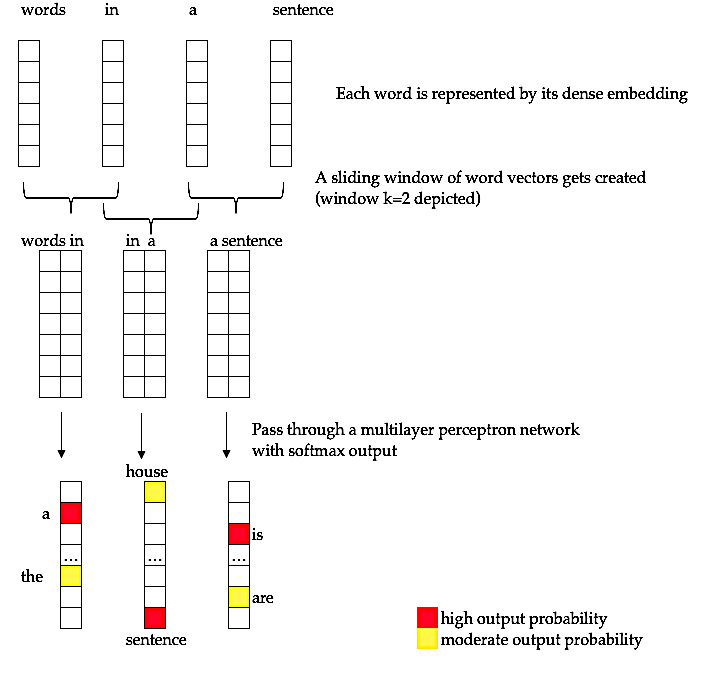
\includegraphics[width=.7\textwidth]{figs/nnlang.png}
    \caption{Diagram for \nameref{sub:nnlm}}
    \label{fig:nnlm}
\end{figure}

\subsection{LSTM}
\label{subsec:lstm}

A concern with our trigram model is that it completely ignores words more than
two positions before the word we wish to predict. To the extent we believe these
words are predictive (personal experience with language suggest that they should
be!), the trigram model has an inherent limitation in its ability to model that
dependence.

One way to combat this is with an LSTM, the architecture of which is depicted in
\cref{fig:lstmdiagram}. At a high level, the LSTM functions by keeping track of
three vectors: $v_t, C_t,$ and $h_t$. The first of these vectors is simply a
dense embedding for the word $w_t$. The $h_t$ and $C_t$ vectors are state
representations of the model, which are dependent on previous words and give the
model a ``memory.'' The LSTM can thus theoretically condition on all previous
text, and in practice exhibits long-term memory through its architecture on
$C_t$ which encourages only intentional changes over time.

The LSTM is formally characterized by the following equations which determine
the evolution of these vectors,

\begin{align}
f_t &= \sigma(W_f \cdot [h_{t-1}, x_t] + b_f) \\
i_t &= \sigma(W_i \cdot [h_{t-1}, x_t] + b_i) \\
\tilde C_t &= \tanh(W_c \cdot [h_{t-1}, x_t] + b_c) \\
C_t &= f_t \odot C_{t-1} + i_t \odot \tilde C_t \\
o_t &= \sigma(W_o [h_{t-1}, x_t] + b_o) \\
h_t &= o_t \odot \tanh(C_t)
\end{align}

Roughly speaking, their intuitions are as follows: $\tilde C_t$ represents the
new information that might be relevant for encoding into long-term memory. $f_t$
captures the information that needs to be deleted from long-term memory, and
$i_t$ captures the places where information needs to be added. Then, these are
combined to determine the new $C_t$. The hidden state roughly captures a
filtered version (captured by the multiplication with $o_t$) of the cell-state.

\begin{figure}[htb]
\centering
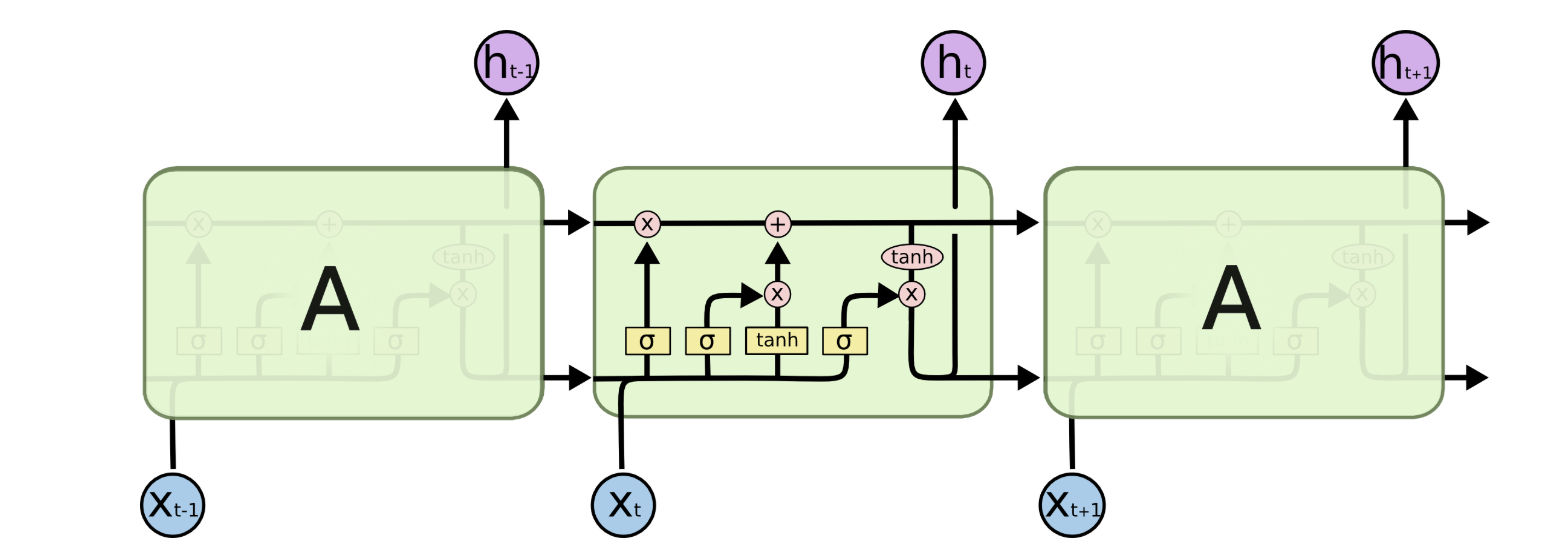
\includegraphics[width=\textwidth]{figs/lstm-diagram.png}
\caption{Depiction of LSTM inner-workings \citep{olah2015understanding}}
\label{fig:lstmdiagram}
\end{figure}

\subsection{Multi-head Attention}
\label{sub:attn}

Following \cite{vaswani2017attention}, we implement a variant of the multi-head
attention
decoder network. Instead of passing the last hidden state from an LSTM $h_t$ to
predict $h_{t+1}$, we use a concatenation of $h_t$ and a \emph{context vector}
$c_t = a_1 h_1 + \cdots + a_{t-1} h_{t-1}$ for \emph{attention values}
$a_1,\ldots, a_{t-1}$ residing in the unit simplex. Following 
\cite{vaswani2017attention}, we use the \emph{scaled attention} mechanism,
where \[
\bm a = \softmax\pr{\br{\frac{h_i^T h_t}{\sqrt{\dim(h_t)}}}_{i=1}^{t-1}}.
\]
In \emph{multi-head attention}, we repeat the attention mechanism above on
different linear projections of $h_1,\ldots,h_t$, with the motivation being that
we wish to capture similarity on different projections of words---one attention
layer could be capturing grammar, another semantics, a third pronoun
association, etc. We depict the architecture in \Cref{fig:attn}, for $t=3$ and
predicting $t+1$.
\begin{figure}[tb]
    \centering
    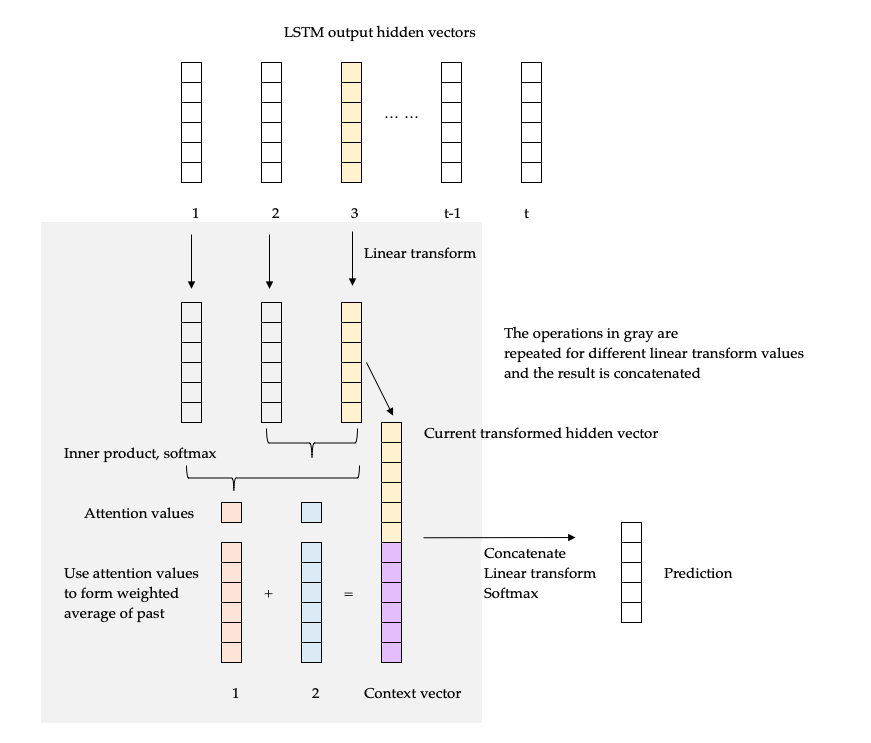
\includegraphics[width=\textwidth]{figs/attention.png}
    \caption{Diagram for \nameref{sub:attn}. In this diagram, we predict the
    fourth word in the sentence by conditioning on the first three. We compute
    attention values of $h_3$ with $h_2$ and $h_1$ and concatenate $h_3$ with a
    context vector $a_1 h_1 + a_2 h_2$, where $a_i$ are the attention values.
    We pass the resulting vector through a linear transformation and softmax
    output. In multi-head attention, we repeat the process for different
    projections of $h_1,h_2,h_3$ and concatenate the results.}
    \label{fig:attn}
\end{figure}

Certain computational tricks need to be employed for efficient utilization of
the GPU. Unlike the encoding attention network, the decoder cannot condition on
future information when predicting the future. As a result, each attention layer
can only look at past hidden states. We parallelize the procedure and take
advantage of GPU hardware by applying attention as usual, computing every
inner product $h_i^T h_j$ for all $i,j$, and use a mask that sets entries with
$h_i^T h_j$
to $-\infty$ if $j \le i$ (which correspond to the forbidden attention
links by looking ahead) before applying the softmax. 

\section{Experiments}
\section{Conclusion}


\bibliographystyle{apalike}
\bibliography{writeup}

\appendix
\section{Model implementation}

\lstinputlisting[caption=Trigram model implementation]{models/trigram.py}
\lstinputlisting[caption=NNLM]
{models/neural_net_lang.py}
\lstinputlisting[caption=LSTM]{models/lstm.py}
\lstinputlisting[caption=LSTM-attention]{models/lstm_att.py}
\lstinputlisting[caption=Ensemble]{models/ensemble.py}




\end{document}
